\documentclass{article}

\usepackage{hyperref}               % Use hyperlinks

\usepackage[T1]{fontenc}            % Codificação para português 
\usepackage[portuguese]{babel}      % Português


\usepackage{algorithm}              % Pseudocódigo
\usepackage[noend]{algpseudocode}

\usepackage{graphicx}               % Coloque figuras
\usepackage{float}                  % Figuras no lugar "esperado"
\graphicspath{{./images/}}          % Localização das imagens

\usepackage{amsmath}                % Use equações alinhadas

\usepackage{enumitem}               % Corrige indentação dentro de enumerates/itemizes
\setlist{  listparindent=\parindent, parsep=0pt, }

\usepackage{hyphenat}               % Use hifens corretamente
\hyphenation{mate-mática recu-perar}

\author{
    Gabriel Rocha Martins
    \and 
    Igor Lacerda Faria da Silva
    \and 
    Luis Felipe Ramos Ferreira
}
\title{Trabalho Prático I \\
Algoritmos II}
\date{% 
}

\begin{document}

\maketitle

\section{Introdução}

\section{Implementação}
O trabalho foi feito inteiramente na linguagem de programação Python, versão 3.10.6, no sistema operacional Ubuntu.

Uma abordagem orientada a objetos foi feita para a realização do trabalho como um todo, uma vez que isso permite um maior controle sobre as funcionalidades implementadas, além de tornar o código mais organizado e bem distribuído.

\subsection{Classes}
Como comentado acima, utilizamos uma abordagem orientada à objetos na implementação do trabalho, e portanto aqui descreveremos as classes que criamos e de que forma foram utilizadas.

\subsubsection{Point}

A classe \texttt{Point} foi criada para representar os pontos bidimensionais que estarão presentes no plano cartesiano. Cada instância da classe é representada por seus dois atributos, o par \( (x,y) \), que representa as coordenadas de valores reais onde os pontos estão localizados.

Na classe, foram implementadas também a sobrecarga de alguns operadores, de modo que a operação sobre os pontos fosse mais ágil. Definimos, principalmente, as comparações entre instância do tipo \texttt{Point}, de modo que:

\begin{itemize}
	\item Um ponto é igual ao outro se suas coordenadas são iguais.
	\item Um ponto é diferente do outro se alguma de suas coordenadas for diferente.
	\item Um ponto é menor que o outro se possuir uma coordenada \( y \) menor, e, caso seja igual, consideramos a menor coordenada \( x \).
	\item Um ponto é maior que o outro se possuir uma coordenada \( y \) maior e, caso seja igual, consideramos a maior coordenada \( x \).
\end{itemize}

Também foi implementado um método que calcula a distância euclidiana entre os dois pontos. O cálculo desse valor é importante para implementações no decorrer do trabalho.

Tais especificações definem a classe de um modo geral, cuja implementação facilitou muito as manipulações feitas nas outras partes do trabalho.

\subsubsection{Segment}

A classe \texttt{Segment} foi criada para representar os segmentos de reta no Plano Cartesiano. Cada instância é representada por dois pontos (instâncias da classe \texttt{Point}), \( p_0 \) e \( p_1 \), os quais representam o ponto de início do segmento e o ponto de fim do segmento, respectivamente.

Essa definição de pontos de início e fim é importante para definirmos o sentido do vetor representado pelo segmento. Além disso, nesse sentido, temos os atributos \( x \) e \( y \) do segmento, que representam os valores de \( x \) e \( y \) referentes ao vetor citado. Dessa forma, podemos definir \( x \) e \( y \) como:

\begin{align*}
	x & = p_1.x - p_0.x \\
	y & = p_1.y - p_0.y
\end{align*}

Em relação às funcionalidades auxiliares, foram implementados métodos para as seguintes utilidades na classe:

\begin{itemize}
	\item Cálculo do produto vetorial entre duas instâncias de um segmento.
	\item Checar se um segmento está em um sentido horário ou anti horário em relação ao outro. Aqui, é importante dizer que, para este trabalho em específico, se dois segmentos são colineares, consideramos que aquele com menor norma como em sentido anti horário em relação ao outro.
	\item Checar se os segmentos são colineares.
	\item Gerar o segmento inverso do atual, isto é, o segmento com mesma norma, direção, mas sentido inverso.
	\item Inverter o próprio segmento, segundo o que foi especificado no item anterior.
	\item Checar se um ponto está no intervalo aberto do segmento.
	\item Checar se um ponto é colinear, está orientado no sentido horário ou anti-horário em relação ao segmento.
	\item Checar se um segmento intersecta outro.
\end{itemize}

Assim como na classe \texttt{Point}, foi feita a sobrecarga de operadores para facilitar as implementações do trabalho. Mais especificamente, sobrecarregamos o comparador de ``menor que'', de modo que um segmento é menor que o outro se este está em sentido horário em relação ao outro.

\subsubsection{ConvexHull}

A implementação do cálculo da envoltória convexa foi, de forma geral, talvez a tarefa que menos demandou esforço entre todas aquelas do trabalho. Isso não quer dizer, no entanto, que ela foi fácil. Apesar de termos à nossa disposição os pseudocódigos dos algoritmos estudados, além de uma gama enorme de implementações na web, compreender os algoritmos ao seu máximo e escrever um código limpo e eficiente que os compute exigiu grande empenho.

Para computarmos, então, a envoltória convexa de um conjunto de pontos, levando em consideração as especificações do trabalho, foi criada uma classe chamada \texttt{ConvexHull}, a qual o construtor demanda um conjunto de pontos cuja envoltória convexa deve ser encontrada.

O segundo parâmetro desse construtor define qual o algoritmo que deve ser utilizado para o cálculo da envoltória. Para este trabalho, implementamos o algoritmo de embrulho de presente, de R.A. Jarvis, o algoritmo da varredura de Graham, de Ronald Graham, e o algoritmo incremental. Efetivamente para o restante do trabalho, utilizamos a varredura de Graham. Nesta seção, apresentaremos as principais diferenças entre as duas abordagens, focando principalmente nas diferenças de tempo de execução notadas para conjuntos de pontos gerados aleatoriamente pela biblioteca \texttt{random} da linguagem Python e para o conjunto de dados utilizados no trabalho.

\begin{enumerate}
	\item \textbf{Algoritmo de embrulho de presente}

	      Como vimos e estudamos em sala de aula, este algoritmo possui uma complexidade de tempo sensível à saída, isto é, ela depende da quantidade de vértices que a envoltória terá ao final da computação. Mais especificamente, a complexidade pertence a \( \Theta(hn) \), onde \( h \) seria o número de vértices citado.

	      Assim como discutimos, também em sala de aula, se o valor de \( h \) tender a \( n \), teremos um algoritmo pouquíssimo eficiente, com uma complexidade quadrática. No entanto, em um caso médio, podemos assumir que \( h \) não assume valores muito grandes, o que tornaria o algoritmo praticamente linear.

	      Claro, assumir isso pode ser perigoso, por isso decidimos comparar os tempos de execução de todos os algoritmos para podermos decidir qual era a melhor opção.

	\item \textbf{Algoritmo da varredura de Graham}

	      O gargalo da complexidade do algoritmo da varredura de Graham está no fato de que os pontos do conjunto inicial devem ser ordenados de acordo com o ângulo polar em relação ao ponto âncora, o que gera um complexidade da ordem de \( \Theta(n \log n) \).

	      No entanto, isso traz certa previsibilidade ao código como um todo. Sabemos que esse sempre será o gargalo do tempo de execução do algoritmo, e certamente é uma das melhores opções quando desejamos estabilidade.

	\item \textbf{Algoritmo incremental}

	      Esse foi, sem sombra de dúvida, o mais difícil de implementar entre os três. Nossa implementação, inclusive, possui alguns \textit{bugs} pontuais, os quais não conseguimos corrigir, por isso mantivemos o uso dos outros dois no trabalho, embora a tentativa de implementação tenha sido muito útil para os estudos.

	      A principal dificuldade, de modo geral, foi decidir qual aresta da envoltória atual deveria ser eliminada ao inserir um novo ponto. No entanto, ao final, conseguimos contornar o problema utilizando as primitivas de orientação de segmentos, podendo assim decidir qual era a melhor opção para cada cenário.

	      O algoritmo incremental, assim como o anterior, possui um gargalo de complexidade provido pela ordenação dos pontos do conjunto inicial em relação à sua coordenada \( x \), além de prover grande estabilidade ao código como um todo.
\end{enumerate}

Abaixo, podemos ver gráficos que demonstram como os diferentes algoritmos se comportaram para pontos gerados aleatoriamente no eixo das coordenadas. A randomicidade dos pontos foi feita por meio da biblioteca \textit{random}, da linguagem Python, e portanto nenhuma distribuição de probabilidade específica afetou esses valores. Geramos, então, para conjuntos variando entre 3 pontos e 100 pontos, 100 envoltórias, e pegamos a média do tempo de geração delas, para cada algoritmo. Tivemos o seguinte gráfico como resultado.

\begin{figure} [H]
	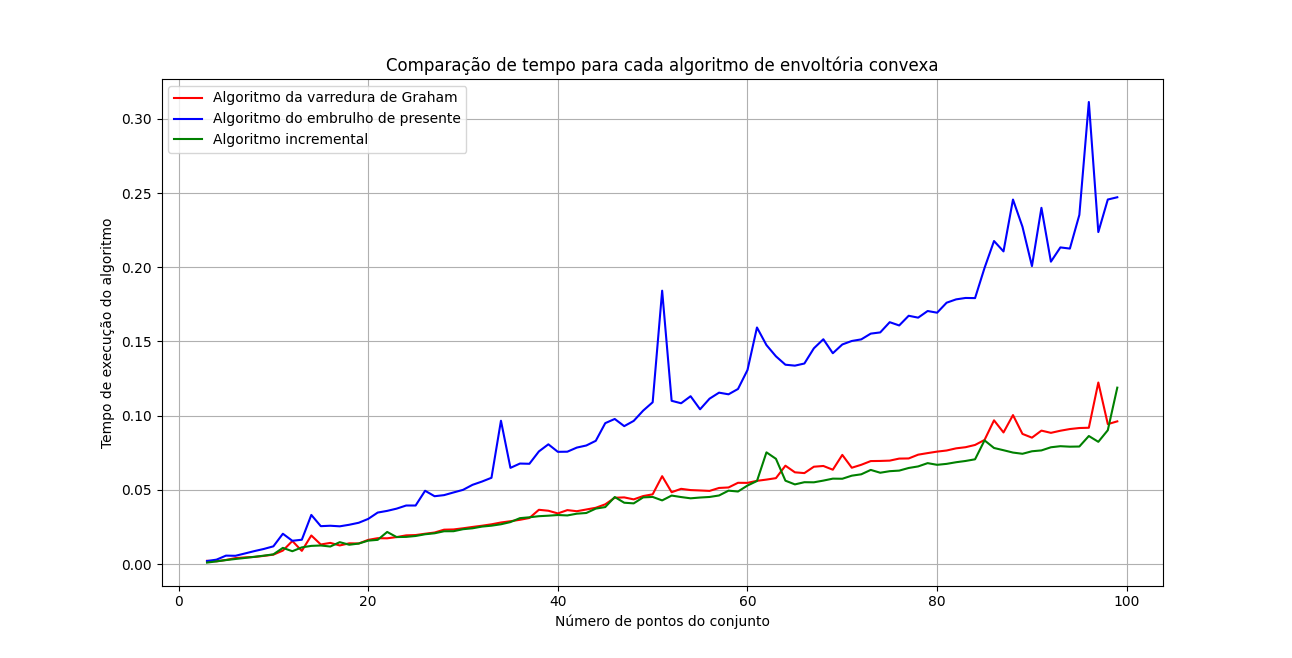
\includegraphics[width=12cm]{uniform.png}
	\centering
\end{figure}

O mesmo foi feito para pontos gerados aleatoriamente por uma distribuição exponencial, por meio da biblioteca \texttt{numpy}, com parâmetro escalar igual a \( \frac{1}{50} \), e obtivemos o seguinte resultado.

\begin{figure} [H]
	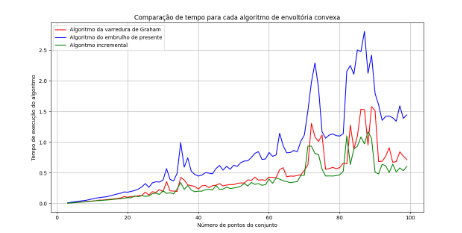
\includegraphics[width=9cm]{exponential.png}
	\centering
\end{figure}

Mais uma vez, tentamos uma distribuição diferente, disponível na biblioteca \texttt{numpy}, e desta vez geramos os pontos com uma distribuição normal de probabilidade, com média 50 e desvio padrão 10. O resultado segue abaixo:

\begin{figure} [H]
	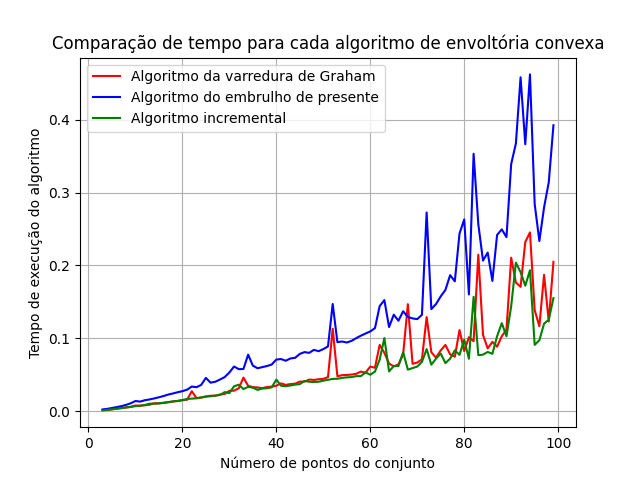
\includegraphics[width=9cm]{normal.png}
	\centering
\end{figure}

Podemos notar que em todos os casos o algoritmo incremental e o algoritmo da varredura de Graham tiveram tempos de execução muito similares, enquanto o algoritmo de embrulho de presente, por possuir pouca estabilidade e ser sensível à saída, teve um desempenho bem abaixo dos outros. Devemos, no entanto, analisar como cada um dos algoritmos se sai na prática com os pontos coletados pelo conjunto de dados que usaremos no trabalho.

De qualquer modo, podemos notar que eles seguem um padrão exatamente como esperávamos. A varredura de Graham e o algoritmo incremental, ambos com a mesma complexidade \( \Theta(n \log n) \), tiveram tempos de execução semelhantes para os testes feitos, enquanto o algoritmo do embrulho de presente demorou muito mais, dado sua inconsistência e sensibilidade à saída.

Após essas análises concluímos então que a melhor opção para utilizarmos no trabalho prático seria o algoritmo da varredura de Graham, uma vez que ela passou em todos os testes que criamos e apresentou um desempenho eficiente e consistente neles.

\subsubsection{LineSweep}

\subsubsection{AlgorithmVisualization}

A classe AlgorithmVisualization não faz parte do escopo do trabalho, e foi feita apenas para que pudessemos visualizar bem como os algoritmos estavam sendo executados, além de auxiliar na correção de bugs encontrados ao longo da execução.

Utilizamos a biblioteca Pygame, uma biblioteca da inguagem Pyhton destinada à criação de jogos simples, para a criação dessas animações. Optamos em utilizá-la para isso pois alguns integrantes da equipe já tinham familiaridade com a tecnologia e porque sua documentação é bem completa.

Todas as animações feitas foram dos três algoritmos de cálculo da envoltória convexa citados anteriormente. De forma geral, podemos dizer que ver uma animação da execução dos algoritmos foi crucial para que erros fossem identificados e conseguíssemos corrigir os bugs. 

Não vamos nos estender muito em realção à documentação dessa classe, visto que ela não fazia parte das definições no enunciado do trabalho. No entanto, deixaremos anexo à esta documentação um vídeo gravado por um de nossos integrantes demonstrando a visualização da execução dos algoritmos, além de que deixaremos ao final desta documentação instruções caso queiram rodar as animações localmente.

\section{Análise experimental dos dados}

\subsection{Processamento dos dados}

\subsection{Treinamento do classificador}

\subsection{Análise de métricas}

\subsection{Resultados}

\section{Conclusão}

\section{Referências Bibliográficas}


\end{document}